\documentclass[a4j]{jarticle}
\usepackage{amsmath}
\usepackage{ascmac}
\usepackage{amssymb}
\usepackage{enumerate}
\usepackage{multicol}
\usepackage{framed}
\usepackage{fancyhdr}
\usepackage{latexsym}
\usepackage{indent}
\usepackage{cases}
\usepackage{wrapfig}
\usepackage[dvipdfmx]{graphics}
\allowdisplaybreaks
\pagestyle{fancy}
\lhead{}
\chead{}
\rhead{東京大学前期$1987$年$2$番}
\begin{document}
%分数関係


\def\tfrac#1#2{{\textstyle\frac{#1}{#2}}} %数式中で文中表示の分数を使う時


%Σ関係

\def\dsum#1#2{{\displaystyle\sum_{#1}^{#2}}} %文中で数式表示のΣを使う時


%ベクトル関係


\def\vector#1{\overrightarrow{#1}}  %ベクトルを表現したいとき(aベクトルを表現するときは\ver
\def\norm#1{|\overrightarrow{#1}|} %ベクトルの絶対値
\def\vtwo#1#2{ \left(%
      \begin{array}{c}%
      #1 \\%
      #2 \\%
      \end{array}%
      \right) }                        %2次元ベクトル成分表示
      
      \def\vthree#1#2#3{ \left(
      \begin{array}{c}
      #1 \\
      #2 \\
      #3 \\
      \end{array}
      \right) }                        %3次元ベクトル成分表示



%数列関係


\def\an#1{\verb|{|$#1$\verb|}|}


%極限関係

\def\limit#1#2{\stackrel{#1 \to #2}{\longrightarrow}}   %等式変形からの極限
\def\dlim#1#2{{\displaystyle \lim_{#1\to#2}}} %文中で数式表示の極限を使う



%積分関係

\def\dint#1#2{{\displaystyle \int_{#1}^{#2}}} %文中で数式表示の積分を使う時

\def\ne{\nearrow}
\def\se{\searrow}
\def\nw{\nwarrow}
\def\ne{\nearrow}


%便利なやつ

\def\case#1#2{%
 \[\left\{%
 \begin{array}{l}%
 #1 \\%
 #2%
 \end{array}%
 \right.\] }                           %場合分け
 
\def\1{$\cos\theta=c$,$\sin\theta=s$とおく.}  %cs表示を与える前書きシータ
\def\2{$\cos t=c$,$\sin t=s$とおく.}     %cs表示を与える前書きt
\def\3{$\cos x=c$,$\sin x=s$とおく.}                %cs表示を与える前書きx

\def\fig#1#2#3 {%
\begin{wrapfigure}[#1]{r}{#2 zw}%
\vspace*{-1zh}%
\input{#3}%
\end{wrapfigure} }           %絵の挿入


\def\a{\alpha}   %ギリシャ文字
\def\b{\beta}
\def\g{\gamma}

%問題番号のためのマクロ

\newcounter{nombre} %必須
\renewcommand{\thenombre}{\arabic{nombre}} %任意
\setcounter{nombre}{2} %任意
\newcounter{nombresub}[nombre] %親子関係を定義
\renewcommand{\thenombresub}{\arabic{nombresub}} %任意
\setcounter{nombresub}{0} %任意
\newcommand{\prob}[1][]{\refstepcounter{nombre}#1[問題 \thenombre]}
\newcommand{\probsub}[1][]{\refstepcounter{nombresub}#1(\thenombresub)}


%1-1みたいなカウンタ(todaiとtodaia)
\newcounter{todai}
\setcounter{todai}{0}
\newcounter{todaisub}[todai] 
\setcounter{todaisub}{0} 
\newcommand{\todai}[1][]{\refstepcounter{todai}#1 \thetodai-\thetodaisub}
\newcommand{\todaib}[1][]{\refstepcounter{todai}#1\refstepcounter{todaisub}#1 {\bf [問題 \thetodai.\thetodaisub]}}
\newcommand{\todaia}[1][]{\refstepcounter{todaisub}#1 {\bf [問題 \thetodai.\thetodaisub]}}


     \begin{oframed}
     点$(x,y)$を点$(x+a,y+b)$にうつす平行移動によって曲線$y=x^2$を移動して得られる曲線を$C$とする.$C$と曲線$y=\cfrac{1}{x}$
     ,$x>0$が接するような$a$,$b$を座標とする点$(a,b)$の存在する範囲の概形を図示せよ.
     
     また,この二曲線が接する点以外に共有点を持たないような$a$,$b$の値を求めよ.ただし,二曲線がある点で接するとは,
     その点で共通の接線を持つことである.
     \end{oframed}

\setlength{\columnseprule}{0.4pt}
\begin{multicols}{2}
{\bf[解]} 題意から$C:y=(x-a)^2+b$である.接点の$x$座標を$t_{>0}$とすれば,$\left(\cfrac{1}{x}\right)'=\cfrac{-1}{x^2}$だから,求める条件は,
     \begin{align}
     &\exists t \left\{
          \begin{array}{l}
          t>0 \\
          (t-a)^2+b=\cfrac{1}{t} \\
          2(t-a)=\cfrac{-1}{t^2} 
         \end{array}
    \right. \nonumber\\
     \Longleftrightarrow
     &\exists t \left\{
          \begin{array}{l}
          t>0 \\
          b=\cfrac{1}{t}-\left(\cfrac{-1}{2t^2}\right)^2 \\
          a=t+\cfrac{1}{2t^2} 
         \end{array}
    \right.\nonumber \\
     \Longleftrightarrow
     &\exists t \left\{
          \begin{array}{l}
          t>0 \\
          b=\cfrac{1}{t}-\cfrac{1}{4t^4} \\
          a=t+\cfrac{1}{2t^2} 
         \end{array}
    \right. \label{1}
    \end{align}
従って,$(a,b)$が\eqref{1}で表されるパラメータ曲線上にあればよい.
    \begin{align*}
    a'&=1-\frac{1}{t^3}=\frac{t^3-1}{t^3} \\
    b'&=\frac{-1}{t^2}+\frac{1}{t^5}=\frac{1-t^3}{t^5}
    \end{align*}
だから下表を得る.
    \begin{align*}
         \begin{array}{|c|c|c|c|c|}\hline
         t       & 0 &     &1                                                  &      \\ \hline
         a'     &    &-    &0                                                  &+    \\ \hline
         b'     &    &+   &                                                  0&-     \\ \hline
         (a,b)&    &\nw&\left(\cfrac{3}{2},\cfrac{3}{4}\right)&\se \\ \hline
         \end{array}
     \end{align*}
また,\eqref{1}から極限値は以下のようになる.
     \begin{align*}
     t\to+0\text{のとき}&\left\{
          \begin{array}{l}
          a\to+\infty \\
          b\to-\infty 
          \end{array}
     \right. \\
     t\to+\infty\text{のとき}&\left\{
          \begin{array}{l}
          a\to+\infty \\
          b\to+0 
          \end{array}
     \right.
     \end{align*}
故にグラフの概形は以下.
     \begin{center}  
      \scalebox{.6}{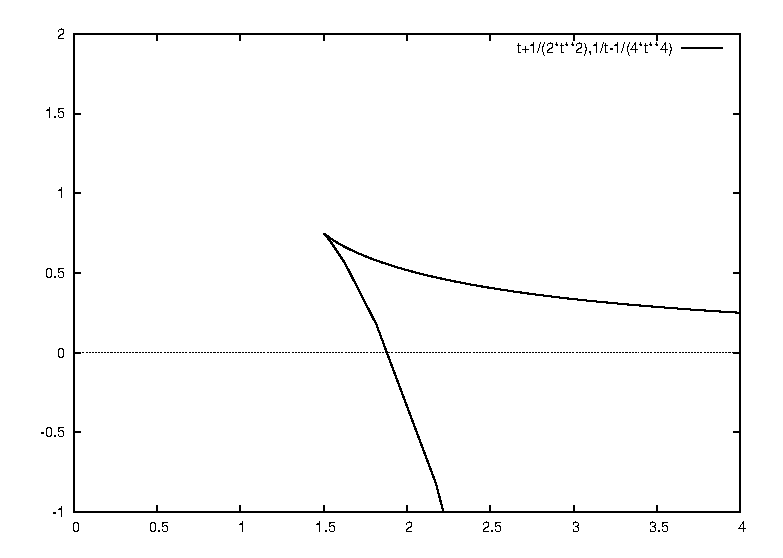
\includegraphics{ut-87-2.eps}}
      \end{center}
次に,接点以外に交点を持たない時,
    \begin{align*}
    (x-a)^2+b=\cfrac{1}{x} 
    \end{align*}
を満たす$x_{>0}$が唯一つ$x=t$のみであればよい.\eqref{1}を代入して
    \begin{align*}
    &\left(x-\left(t+\cfrac{1}{2t^2}\right)\right)^2+\left(\cfrac{1}{t}-\cfrac{1}{4t^4}\right)=\cfrac{1}{x} \\ 
    \Longleftrightarrow%
    &x^2-2\left(t+\cfrac{1}{2t^2}\right)x+\left(t+\cfrac{1}{2t^2}\right)^2+\left(\cfrac{1}{t}-\cfrac{1}{4t^4}\right)=\cfrac{1}{x} \\
    \Longleftrightarrow%
    &x^3-2\left(t+\cfrac{1}{2t^2}\right)x^2+\left(t^2+\cfrac{2}{t}\right)x-1=0 \\
    \Longleftrightarrow%
    &(x-t)^2\left(x-\cfrac{1}{t^2}\right)=0
    \end{align*}
だから,条件は$t>0$も考慮して
     \[t=\cfrac{1}{t^2}\Longleftrightarrow t=1\]
 である.この時,\eqref{1}から,$(a,b)=\left(\dfrac{3}{2},\dfrac{3}{4}\right)$となる.$\cdots$(答)
\newpage
\end{multicols}
\end{document}